\newpage
\chapter{Theory Development}
\section{Introduction}
In the previous chapter, various estimation techniques applied to \ac{Radar} target tracking were reviewed. This chapter establishes the theoretical foundation for the tracking filters developed in this research. Section 3.2 introduces the mathematical foundations of estimation techniques, paving the way for a detailed discussion of the Kalman Filter and the \ac{UKF} in Section 3.3. Section 3.4 discusses the theory behind the \ac{RGNF}, including a thorough derivation and application of its equations. The theory of \ac{PF} is addressed in Section 3.5, beginning with an overview of the fundamental concepts underpinning \ac{PF} theory. Furthermore, Section 3.6 discusses adaptive filtering techniques. Lastly, Section 3.7 introduces the log-likelihood as a statistical benchmark for evaluating the tracking filters.

\section{Target State Estimation Theory}
\ac{Radar} tracking systems are mostly used to measure and estimate the state of the target, which can be the target's range,  elevation angle, azimuth angle, velocity or Doppler frequency, amongst other target parameters. Continuous usage and tracking of these parameters enables the system to estimate their future values. According to Richards \textit{et.al} \cite{Richards2010}, target tracking can be separated into two parts: \textit{a)  Data association for assigning measurements to tracks} and \textit{b) Target estimation with tracking filters}.
\newline
\newline
Measurement-to-track data association involves the assignment and matching of an observation to a corresponding track or the creation of a new track if the detection is from a newly found target, where a track is defined as a collection of values for a single target's state at a specific point in time. In \ac{Radar} or navigation systems, measurements are values that can be extracted from sensors or \ac{Radar} maps such as \ac{CFAR} or range and Doppler maps that have information about the state of the target. The process of measurement-to-track data association can become even more complex due to closely spaced targets, target maneuvers and \ac{Radar} with low resolution, which all make it difficult to classify target measurements and assign them to correct tracks.
\newline
\newline
Track filtering refers to the estimation of a target's trajectory, including its position, velocity, and acceleration amongst other parameters, based on noisy measurements such as range, elevation, and bearing that have been associated with a track \cite{Richards2010}. The estimate of the trajectory from the tracking filter has an uncertainty associated with it that is characterized by the co-variance of the estimate. The predicted position and velocity are then used to estimate the next observation. Figure \ref{fig1:multi-target} illustrates the vital purpose of target tracking in \ac{Radar} systems. In target tracking, a track may denote the position, velocity, or other parameters representing an entity perceived in the environment, while a target is an actual object in the environment that the \ac{Radar} is intended to track. In \cite{Richards2010} it is noted that ``the number of tracks maintained by a \ac{Radar} tracking system can be greater (extra) or fewer (missed) than the actual number of targets''. In a perfect scenario, the number of tracks should match the number of targets. In this section, the fundamentals of single target tracking with a \ac{Radar} are addressed.

In this chapter, the fundamentals of Kinematic State Estimation (track filtering), focusing on two main approaches to filtering algorithms are discussed. The first approach uses deterministic estimation that assumes a perfect model for the target's motion, where the track error covariance approaches zero as more data is processed. In contrast, the second approach uses stochastic state estimation, assuming an imperfect model for the target's motion. In stochastic state estimation, the target's motion model incorporates a random process, and the covariance of the track does not approach zero as more data is processed \cite{Richards2010}.

\begin{figure}[H]
	\centering
	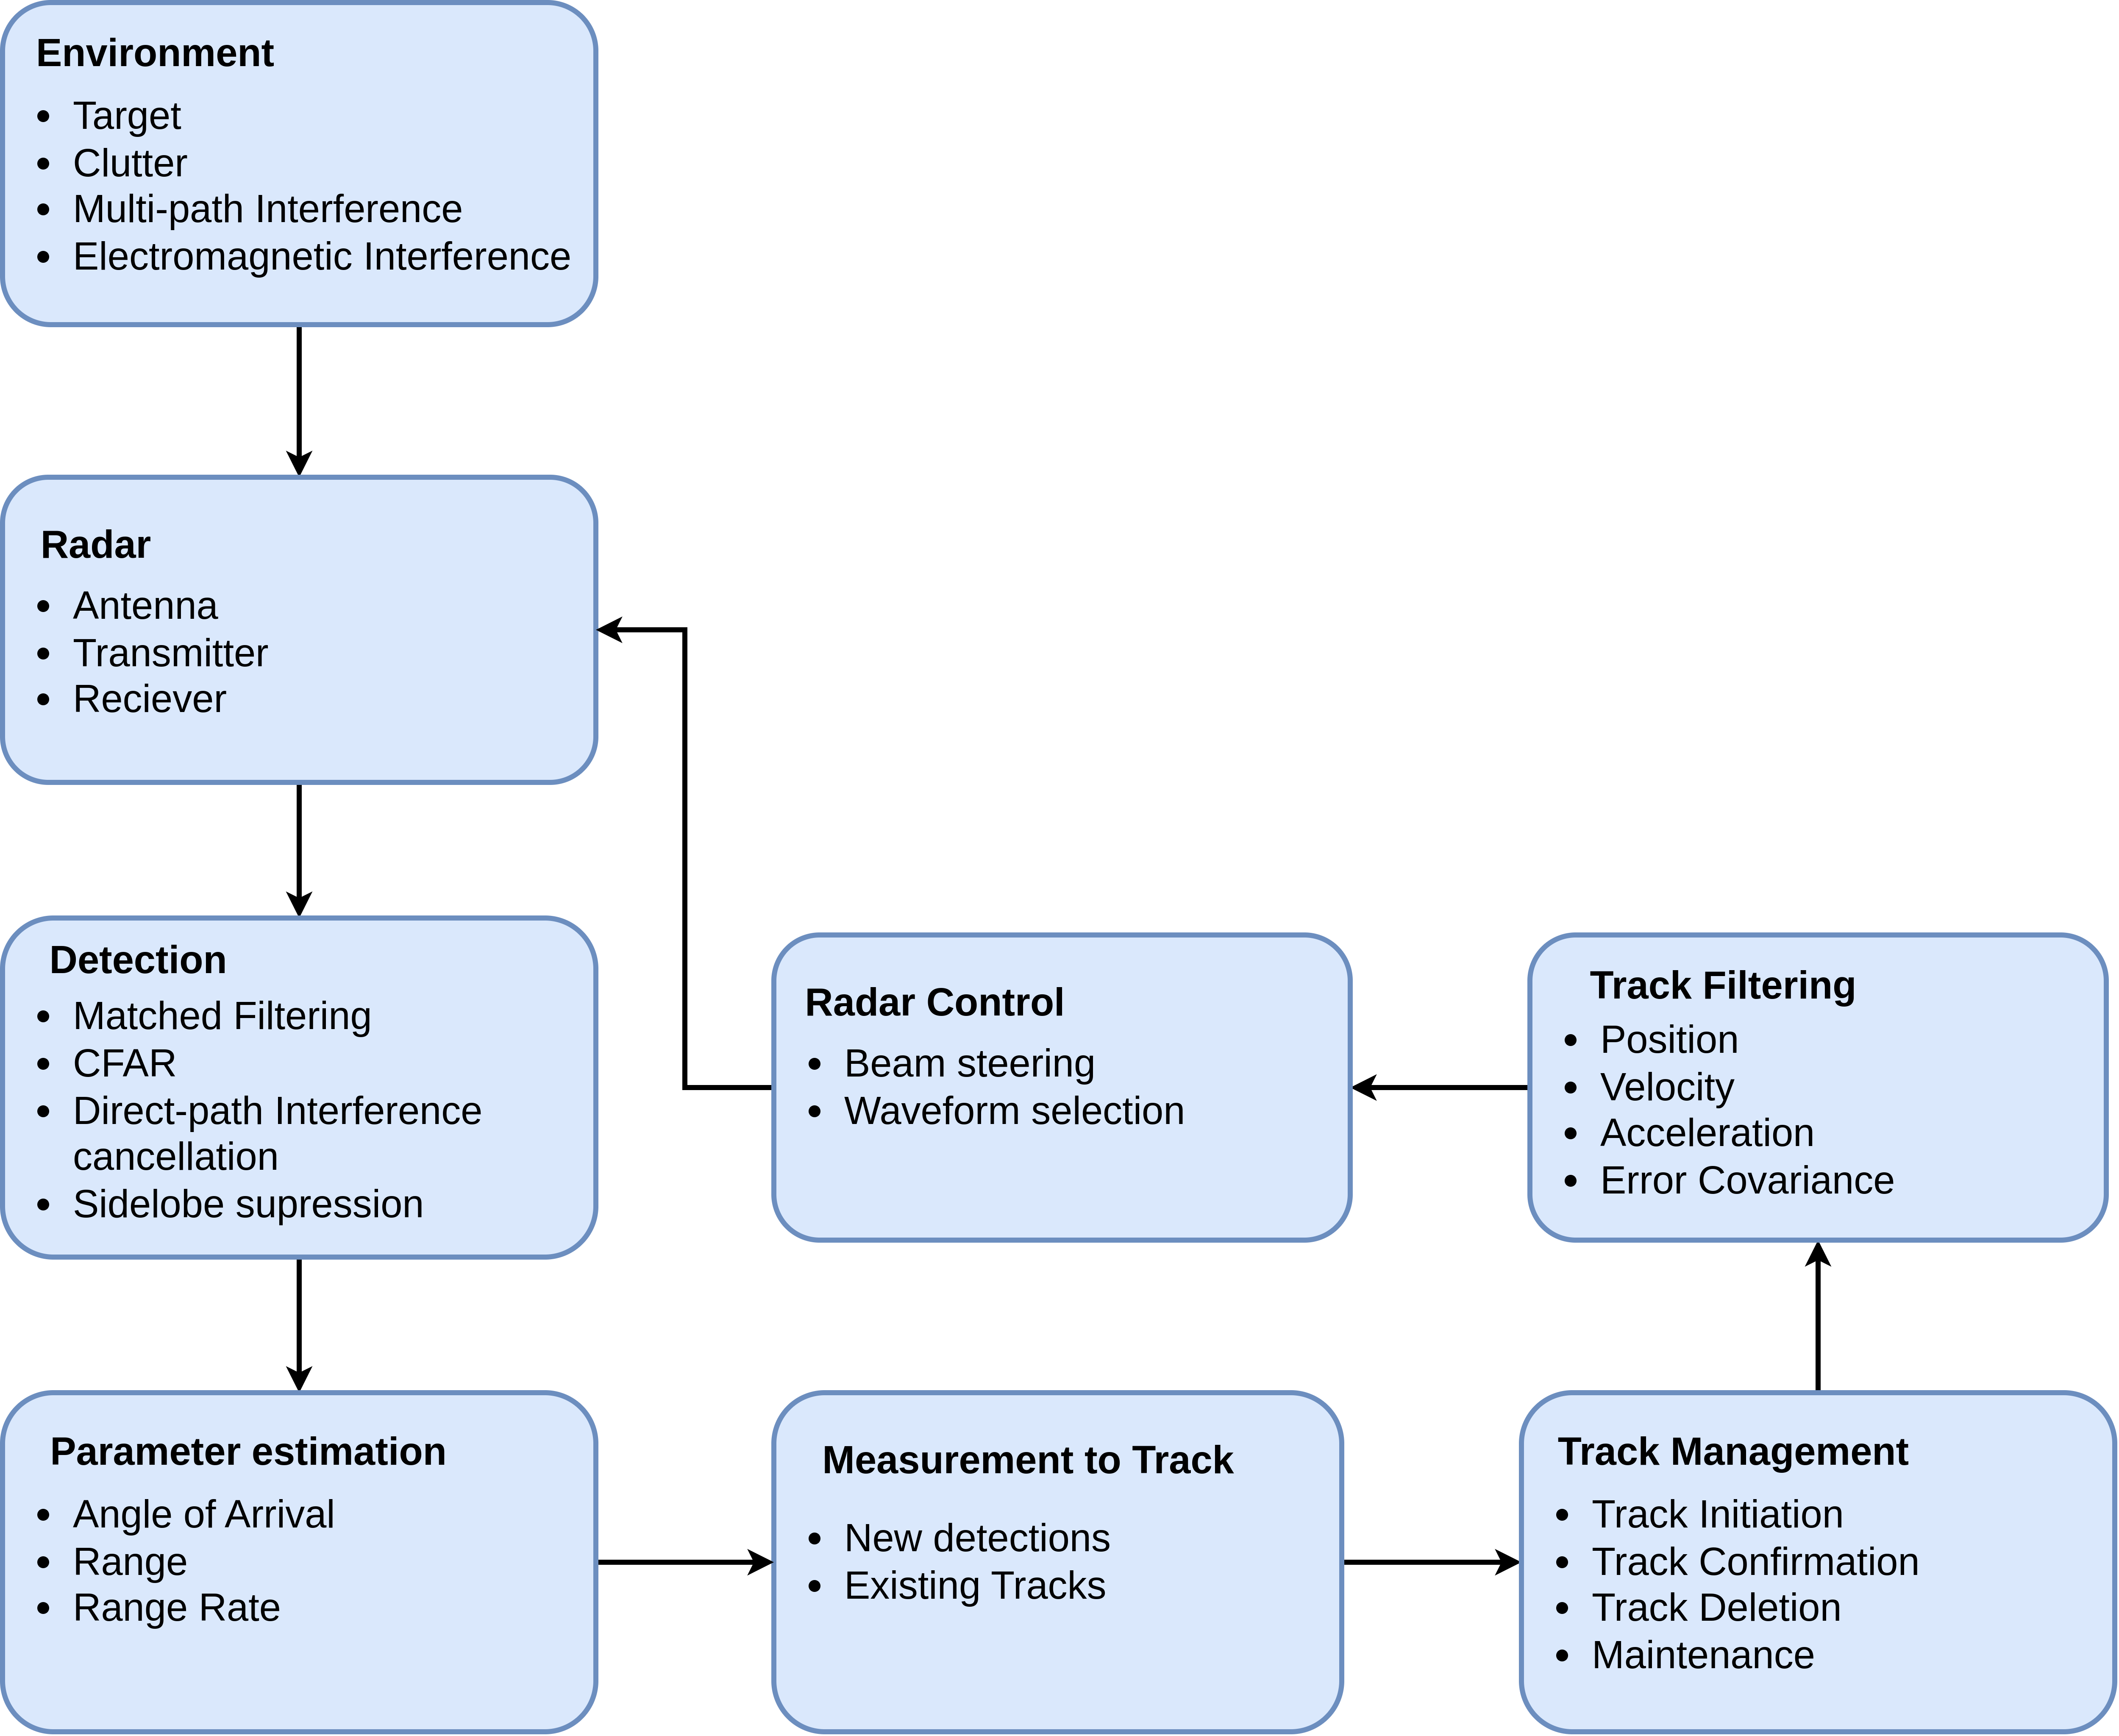
\includegraphics[width=1\linewidth]{Figure/Process.drawio.png}
	\caption{Processing chain for a MTT Radar system.}
	\label{fig1:multi-target}
\end{figure}
%Recursive Bayesian Estimation - TYPES OF Estimators in Estimation Theory%

For stochastic state estimation, the measurements are defined in Equation (\ref{measurement_eq}), the dynamical motion model is given in Equation (\ref{dynamic_model}), and the variables are described in Table \ref{dynamic_model}.
\begin{equation}
    Z_k=H_kX_k+w_k
    \label{measurement_eq}
\end{equation}
\begin{equation}
    X_{k+1} = F_kX_k+G_kv_k
    \label{dynamic_model}
\end{equation}

\begin{table}[ht!]
    \centering
    \large
    \caption{Description of Variables for Stochastic State Estimation.}
    \label{tab:state_estimation_variables}
    \begin{tabular}{lp{12cm}} % Adjust the width (8cm) as needed
        \toprule
        Variable & Description \\
        \midrule
        \( Z_k \)       & Measurement vector at time step \( k \), representing the observed data. \\
        \( H_k \)       & Observation matrix at time step \( k \). \\
        \( X_k \)       & State vector at time step \( k \). \\
        \( w_k \)       & Measurement noise at time step \( k \), typically zero-mean Gaussian noise with covariance \( R_k \). \\
        \( X_{k+1} \)   & Predicted state vector at time step \( k+1 \). \\
        \( F_k \)       & State transition matrix at time step \( k \). \\
        \( G_k \)       & Control input matrix at time step \( k \). \\
        \( v_k \)       & Process noise at time step \( k \), typically zero-mean Gaussian noise with covariance \( Q_k \). \\
        \bottomrule
    \end{tabular}
\end{table}

In a \ac{NCV} motion model, the target's state vector in a scalar coordinate system is described by Equation (\ref{xk}) \cite{Richards2010}. Here $x_k$ represents the target's position at time $t_k$ and $\dot{x_k}$ represents the target's velocity. The process noise is also included to account for uncertainties related to unknown maneuvers and unmodeled dynamics of the target being tracked.
\begin{equation}
    X_k=[x_k\; \dot{x_k}]^T
    \label{xk}
\end{equation}

Malik and Salih\cite{Salih2011} define filtering as the process of ``estimating the state of the system based on measured observations, with the system being represented by its state-space model''. With every new state, the filtering process attempts to estimate the state of the system prior to the measurements. When new measurements become available, the estimation is updated and a new estimation for the next state is calculated \cite{CHEN2}. \textit{Prediction} is a preliminary estimation method that infers the expected value of a quantity at a future time \( t + \tau \) (\( \tau > 0 \)) based on data available up to time \( t \). In the Equations (\ref{1a}) and (\ref{1b}), the generic stochastic filtering problem is considered in a dynamic state-space form.

\begin{equation}
    \dot{x_t} = f(t,x_t,u_t,d_t)
    \label{1a}
\end{equation}
\begin{equation}
        y_t=g(t,x_t,u_t,v_t)
        \label{1b}
\end{equation}

Equations (\ref{1a}) and (\ref{1b}) are known as the state and measurement equations, respectively. Here, \( x_t \) denotes the state vector, \( y_t \) represents the measurement vector, and \( u_t \) is the system input vector in a controlled setting. The terms \( d_t \) and \( v_t \) correspond to process noise and measurement noise, respectively. While the formulation above is in the time domain, discrete-time filtering is typically emphasized in practical applications, as illustrated in Equations (\ref{1c}) and (\ref{1d}).

\begin{equation}
    x_{n+1} = f(x_n,d_n)
    \label{1c}
\end{equation}
\begin{equation}
    y_n=g(x_n,v_n)
    \label{1d}
\end{equation}

In the discrete-time domain, \( d_n \) and \( v_n \) are treated as white noise random sequences with uncertain statistical characteristics. According to Chen \cite{CHEN2}, Equations (\ref{1c}) and (\ref{1d}) simplify to a special case in which a linear Gaussian dynamic system is assumed.
\begin{equation}
    x_{n+1} = F_{n+1},x_n +d_n
    \label{1e}
\end{equation}
\begin{equation}
    y_n=G_nx_n+v_n
    \label{1f}
\end{equation}

The analytic filtering solution is discussed in the Kalman Filtering solution. The Equations (\ref{1e}) and (\ref{1f}) are the transition matrix and measurement matrix respectively.

\section{Kalman Filter Theory}
This section covers the theory and formulation of the Kalman Filter and the \ac{UKF}. It begins with an overview of their frameworks, detailing the mathematical foundations. The algorithms for implementing these filters, namely the prediction and update steps are also discussed in this section. 

\subsection{Kalman Filter}
As noted in the literature, the Kalman Filter algorithm is widely used and useful for estimating the state of a dynamic system based on a sequence of noisy measurements. It is recognized for its efficiency as a recursive, weighted least-squares estimator, assuming that the error statistics follow Gaussian probability distributions \cite{Karlgaard2006}. The Kalman Filter is particularly effective in tracking targets with linear or non-maneuvering trajectories \cite{Bauermeister2016}. The equations governing the Kalman Filter are discussed in the subsequent subsection.

\subsubsection{Principles of Kalman Filtering }
The Kalman Filter is composed of several mathematical equations that define the prediction and the update stage, which operate together as a feedback control mechanism \cite{Adyn}. In the diagram in Figure \ref{fig1:kalmanFilter} from \cite{Adyn}, The Kalman Filter operates by first making a prediction and then applying a correction step to correct and estimate the states of the system. The main idea is that by using information about the state dynamics, the filter forecasts and predicts the subsequent state. As noted in \cite{KalmanTut} a straightforward example is that if I know my previous position (previous state) and my speed (state dynamics), I can estimate my current position (current state).
\begin{figure}[H]
	\centering
	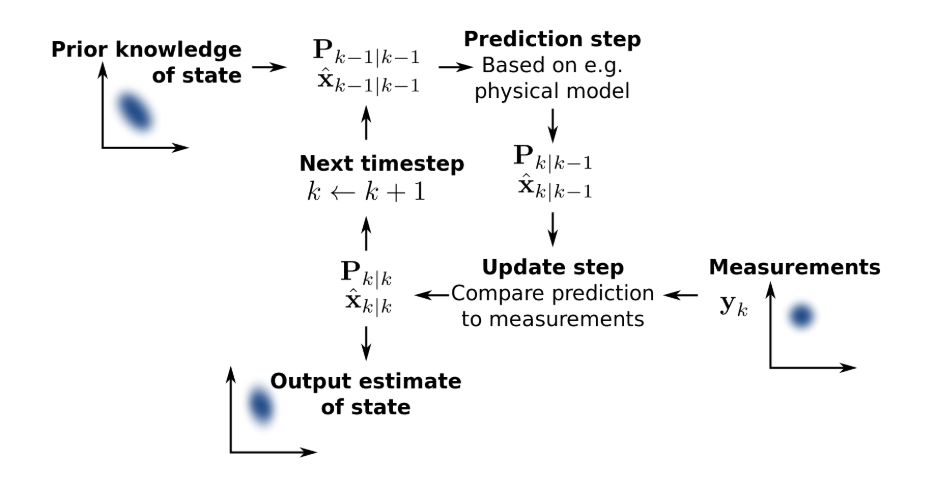
\includegraphics[width=1\linewidth]{Figure/kalmanfilter.PNG}
	\caption{Concept of Kalman Filtering.}
	\label{fig1:kalmanFilter}
\end{figure}

The process model that governs the evolution of the state from time $k-1$ to time $k$ is given by Equation (\ref{kalman_process_model}) :
\begin{equation}
    x_k =Fx_{k-1}+Bu_{k-1} +w_{k-1}
    \label{kalman_process_model}
\end{equation}

Similarly to  \cite{Kim} where $F$ is denoted as the state transition matrix,  whose product with a state vector at an earlier time can give the state at a later time, is applied to the previous state vector $x_{k-1}$. $B$ represents the control-input matrix applied to the control vector $u_{k-1}$, while $w_{k-1}$ is the process noise vector, assumed to follow a zero-mean Gaussian distribution with covariance $Q$.

The process model has a measurement model associated with it, which describes the relationship between the state and the measurement at the current time step k as shown in Equation (\ref{kalman_measure_model}):
\begin{equation}
    z_k=Hx_k+v_k
    \label{kalman_measure_model}
\end{equation}

As described in \cite{Kim}, ``$z_k$ is the measurement vector, H is the measurement matrix, and $v_k$ is the measurement noise vector that is assumed to be zero-mean Gaussian with covariance R i.e.,$v_k \sim  \textit{N}(0,R)$''. Given an initial estimate $x_0$ and a sequence of measurements $\{z_1, z_2, \dots\}$, the system evolution is governed by $F$, $B$, $H$, $Q$, and $R$. The Kalman Filter then uses this information to estimate $x_k$ at time step $k$.


\subsubsection{The Kalman Filter Algorithm}
The Kalman Filter algorithm is composed of two stages: the prediction and update stages. These stages are commonly referred to as the "propagation" and "correction" phases \cite{Kim}.

\paragraph{Kalman Filter Prediction Stage}\mbox{}

The prediction stage involves estimating the state as shown in Equation (\ref{eq:predicted_state}) and error covariance shown in Equation (\ref{eq:predicted_covariance}) at time \( k \) based on the previous state and control input.

\begin{equation}
\hat{x}_k^- = F \hat{x}^+_{k-1} + B u_{k-1}
\label{eq:predicted_state}
\end{equation}
\begin{equation}
P_k^- = F P^+_{k-1} F^T + Q
\label{eq:predicted_covariance}
\end{equation}

\paragraph{Kalman Filter Update Stage}\mbox{}

The update stage refines the predicted estimates using the measurement data, where the Equations in (\ref{eq:measurement_residual})-(\ref{eq:updated_covariance}) are used.

\begin{equation}
\tilde{y}_k = z_k - H \hat{x}^-_k
\label{eq:measurement_residual}
\end{equation}
\begin{equation}
K_k = P^-_k H^T \left( R + H P^-_k H^T \right)^{-1}
\label{eq:kalman_gain}
\end{equation}
\begin{equation}
\hat{x}^+_k = \hat{x}^-_k + K_k \tilde{y}_k
\label{eq:updated_state}
\end{equation}
\begin{equation}
P^+_k = (I - K_k H) P^-_k
\label{eq:updated_covariance}
\end{equation}

In the equations presented in Equations (\ref{eq:predicted_state})-(\ref{eq:updated_covariance}), the hat operator $\hat{}$ is used to denote the estimate of a variable, while the superscripts $-$ and $+$ indicate the predicted and updated estimates respectively. The term $P$ refers to the state error covariance. The covariance of the random variable $x$ is given by $cov(x) = \mathbb{E}[(x-(\hat x)(x-(\hat x)^T]$ where $\mathbb{E}$ represents the expected value operator, which computes the mean of its argument.


During the update process, $\tilde{y}_k$ which represents the measurement residual is first calculated as the difference between the actual measurement $z_k$ and the predicted measurement $H\hat{x}^-_k$. Furthermore, the predicted state is multiplied by the measurement matrix $H$ to estimate the current measurement. To refine the predicted estimate $\hat{x}_k^-$, the residual $y_k$ is scaled by the Kalman gain $K_k$. This results in an updated state estimate. Following this update, the error covariance $P_k^+$ is recomputed.


An effective initialization is crucial for implementing the Kalman Filter successfully. The initial state estimate $\hat{x}^+_0$, the initial error covariance matrix $P^+_0$, and the noise covariance matrices $Q$ and $R$ play a vital role in determining the filter's performance. For instance, selecting a large $P^+_0$ can lead to faster convergence, while incorrect values for the measurement covariance matrix $R$ can adversely affect the integration of measurements. The Kalman Filter algorithm is illustrated in Algorithm \ref{alg:kalman_filter}.\footnote{The Matlab code for the algorithm's implementation can be found in the code repository from Appendix \ref{appendix:repo}.}
\newline
\begin{algorithm}[H]
\caption{Kalman Filter Algorithm for State Estimation.}
\label{alg:kalman_filter}
\begin{algorithmic}[1]
    \vspace{0.6em}
    \State \textbf{Initialize:} $\mathbf{x}_0$, $\mathbf{P}_0$, $\mathbf{Q}$, $\mathbf{R}$
    \vspace{1em}
    
    \State \textbf{Prediction:}
    \vspace{0.6em}
    \State $\mathbf{x}_{k|k-1} \gets \mathbf{A}\mathbf{x}_{k-1|k-1} + \mathbf{B}\mathbf{u}_{k-1}$
    \vspace{0.6em}
    \State $\mathbf{P}_{k|k-1} \gets \mathbf{A}\mathbf{P}_{k-1|k-1}\mathbf{A}^\top + \mathbf{Q}$
    \vspace{1em}
    
    \State \textbf{Update:}
    \vspace{0.6em}
    \State $\mathbf{K}_k \gets \mathbf{P}_{k|k-1}\mathbf{H}^\top(\mathbf{H}\mathbf{P}_{k|k-1}\mathbf{H}^\top + \mathbf{R})^{-1}$
    \vspace{0.6em}
    \If{observation $\mathbf{z}_k$ is available}
        \vspace{0.3em}
        \State $\mathbf{x}_{k|k} \gets \mathbf{x}_{k|k-1} + \mathbf{K}_k(\mathbf{z}_k - \mathbf{H}\mathbf{x}_{k|k-1})$
        \vspace{0.3em}
    \EndIf
    \vspace{0.6em}
    \State $\mathbf{P}_{k|k} \gets (\mathbf{I} - \mathbf{K}_k\mathbf{H})\mathbf{P}_{k|k-1}$
    \vspace{0.6em}
\end{algorithmic}
\end{algorithm}

The Kalman Filter operates under the assumption that both the process and measurement models follow a linear structure, meaning that the relationships between the states, state transitions, and measurements can be expressed using linear equations with the matrices $F$, $B$, and $H$. Additionally, the process and measurement noise are assumed to be additive Gaussian \cite{Kim}. This assumption can be a limitation when the actual observations deviate from the Gaussian assumptions. In the next subsection, a variant of the Kalman Filter designed to handle non-linear models will be discussed.

\subsection{Unscented Kalman Filter}
The implementation of the \ac{UKF} involves the utilization of sampling points known as sigma points. This stands in contrast to the traditional Kalman Filter, where only a singular point (mean) is propagated. In the context of the \ac{UKF}, multiple sigma points are propagated through the linear or non-linear function. This process results in a more accurate recovery of the mean and covariance of the state.
\begin{figure}[H]
	\centering
	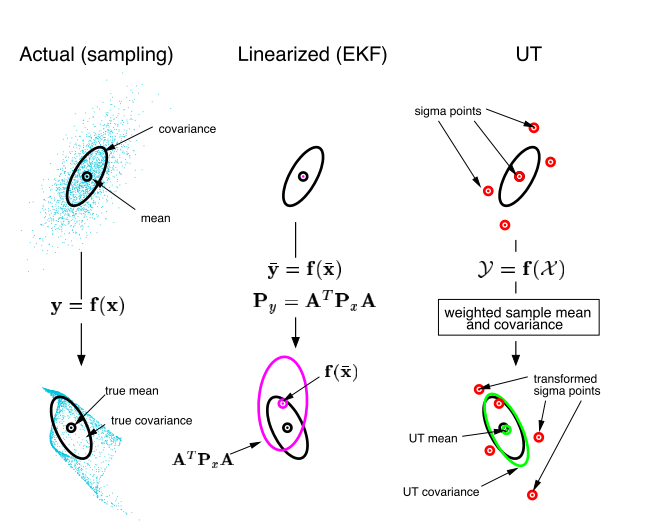
\includegraphics[width=1.1\linewidth]{Figure/UKF.png}
	\caption{Comparison of Monte Carlo methods, EKF, and UKF processes. Left: Monte Carlo sampling representing actual distribution, Middle: Linearized EKF approach, Right: UT applied in the UKF.}
	\label{fig1:UKF}
\end{figure}

\noindent  This approach to filtering diverges from conventional sampling techniques like Monte Carlo methods, including particle filtering, which require a significant number of sample points in order to propagate an accurate distribution of the state \cite{Cai2006}. 
Figure  \ref{fig1:UKF} from \cite{Cai2006} demonstrates how the true mean and covariance evolve in a two-dimensional (2D) system, with Monte Carlo sampling results shown in the left plot; the \ac{EKF} method which uses the linearisation approach is shown in the centre and the right plot shows the \ac{UT} of the \ac{UKF} where only 5 sigma points are necessary for a \ac{2D} system.

In \cite{Julier1997a}, the \ac{UT} is defined as a technique for deriving ``the statistics of a random variable subjected to a non-linear transformation''. It operates on the premise that approximating a Gaussian distribution is simpler than approximating a non-linear function or transformation. By considering the propagation of a random variable \( \mathbf{x} \) with a vector of dimension \( \mathbf{L} \) through a non-linear mapping \( \mathbf{y} = g(\mathbf{x}) \), where \( \mathbf{x} \) has a mean \( \bar{\mathbf{x}} \) and covariance \( \mathbf{P}_x \)  \cite{Cai2006}. The statistics of \( \mathbf{y} \) can be derived using the matrix  \( \mathcal{X} \) of  2\(L\)+1 sigma vectors \( \mathcal{X}_i \) with corresponding weights   \(W_i\) as shown in Equations in (\ref{ukf_equations1}) - (\ref{ukf_equations2}).

\begin{equation}
\begin{aligned}
    \mathcal{X}_0 &= \bar{\mathbf{x}} \\
    \mathcal{X}_i &= \bar{\mathbf{x}} + \left(\sqrt{(L+\lambda)\mathbf{P}_x}\right)_i \quad i = 1,\ldots,L \\
    \mathcal{X}_i &= \bar{\mathbf{x}} + \left(\sqrt{(L+\lambda)\mathbf{P}_x}\right)_{i-L} \quad i = L+1,\ldots,2L
\end{aligned}
\label{ukf_equations1}
\end{equation}

\begin{equation}
\begin{aligned}
    W^{(c)}_0 &= \lambda / (L + \lambda) + (1-\alpha^2 +\beta) \\
    W^{(m)}_0 &= \lambda / (L + \lambda) \\
    W^{(m)}_i &= W^{(c)}_i  = 1/\{2(L + \lambda)\}, \quad i = 1,\ldots,2L\\    
\end{aligned}
\label{ukf_equations2}
\end{equation}

\begin{equation}
\begin{aligned}
    \lambda = \alpha^2(L+\kappa) - L
    \label{lambdaequation}
\end{aligned}
\end{equation}

\(\lambda\) is computed using the Equation in (\ref{lambdaequation}) and all the parameters are described in Table \ref{tab:ukf_parameters}. The \( i \)th row of the square root matrix, denoted as \( \left(\sqrt{(L+\lambda)\mathbf{P}_x}\right)_i \), is used to construct the sigma vectors, which are then passed through the non-linear function shown in Equation (\ref{nonlinear}).


\begin{equation}
    \begin{aligned}
        \mathcal{Y}_i = g(\mathcal{X}_i) \quad i = 0,\ldots,2L
    \end{aligned}
    \label{nonlinear}
\end{equation}

\begin{table}[H]
    \centering
    \large
    \caption{Parameters for Unscented Kalman Filter.}
    \label{tab:ukf_parameters}
    \begin{tabular}{ll}
        \toprule
        Parameter & Description \\
        \midrule
        \( \mathcal{X}_0 \) & Initial sigma point \\
        \( \mathcal{X}_i \) & Sigma points \\
        \( W^{(m)}_i \) & Weight for mean \\
        \( W^{(c)}_i \) & Weight for covariance \\
        \( \lambda \) & Scaling factor \\
        \( \kappa \) & Secondary scaling factor \\
        \( \alpha \) & Distribution of sigma points \\
        \( \beta \) & Incorporation of prior knowledge \\
        \bottomrule
    \end{tabular}
\end{table}
\noindent As stated in \cite{Julier1997a}, ``the mean and covariance for \( \mathbf{y} \) are estimated using a weighted sample mean and covariance of the posterior sigma points,'' as shown in Equations (\ref{equkf1}) and (\ref{equkf2}).  
\begin{equation}
    \begin{aligned}
        \bar{\mathbf{y}} \approx \sum_{i=0}^{2L} W^{(m)}_i \mathcal{Y}_i
    \end{aligned}
    \label{equkf1}
\end{equation}
\begin{equation}
    \begin{aligned}
        \mathbf{P}_x \approx \sum_{i=0}^{2L} W^{(c)}_i \{\mathcal{Y}_i-\bar{\mathbf{y}}\}\{\mathcal{Y}_i-\bar{\mathbf{y}}\}^T
    \end{aligned}
    \label{equkf2}
\end{equation}
\subsubsection{Unscented Kalman Filter Algorithm}
Similar to the Kalman Filter, the \ac{UKF} follows a similar approach to the Kalman filter's state estimation, consisting of the prediction and update stages.

\paragraph{Prediction Stage}\mbox{}

The prediction stage involves creating sigma points, predicting sigma points, computing the predicted state estimate, and calculating the predicted error covariance, as shown in Equations (\ref{eq:create_sigma_points}) to (\ref{eq:predicted_covariance_ukf}) respectively.

\begin{equation}
\mathbf{X}^a_{k-1} = \left[\hat{\mathbf{x}}^a_{k-1} \quad \hat{\mathbf{x}}^a_{k-1} \pm \sqrt{(L+\lambda)\mathbf{P}^a_{k-1}}\right]
\label{eq:create_sigma_points}
\end{equation}
\begin{equation}
\mathbf{X}^x_{k|k-1} = \mathcal{F}\left[\mathbf{X}^x_{k-1}, \mathbf{X}^v_{k-1}\right]
\label{eq:predict_sigma_points}
\end{equation}
\begin{equation}
\hat{\mathbf{x}}^-_k = \sum_{i=0}^{2L} W^{(m)}_i \mathbf{X}^x_{i,k|k-1}
\label{eq:predicted_state_ukf}
\end{equation}
\begin{equation}
\mathbf{P}^-_k = \sum_{i=0}^{2L} W^{(c)}_i \left[\mathbf{X}^x_{i,k|k-1} - \hat{\mathbf{x}}^-_k\right]\left[\mathbf{X}^x_{i,k|k-1} - \hat{\mathbf{x}}^-_k\right]^T
\label{eq:predicted_covariance_ukf}
\end{equation}

\paragraph{Update Stage}\mbox{}

The update stage involves calculating the predicted measurements, the predicted measurement estimate, the innovation covariance, the cross-covariance, the Kalman gain, the updated state estimate, and the revised error covariance, as shown in Equations (\ref{eq:predicted_measurement}) - (\ref{eq:updated_covariance_ukf}) respectively.

\begin{equation}
\mathbf{Y}_{k|k-1} = \mathcal{H}\left[\mathbf{X}^x_{k|k-1}, \mathbf{X}^n_{k-1}\right]
\label{eq:predicted_measurement}
\end{equation}
\begin{equation}
\hat{\mathbf{y}}^-_k = \sum_{i=0}^{2L} W^{(m)}_i \mathbf{Y}_{i,k|k-1}
\label{eq:predicted_measurement_estimate}
\end{equation}
\begin{equation}
\mathbf{P}_{\tilde{y}_k\tilde{y}_k} = \sum_{i=0}^{2L} W^{(c)}_i \left[\mathbf{Y}_{i,k|k-1} - \hat{\mathbf{y}}^-_k\right]\left[\mathbf{Y}_{i,k|k-1} - \hat{\mathbf{y}}^-_k\right]^T
\label{eq:innovation_covariance}
\end{equation}
\begin{equation}
\mathbf{P}_{\mathbf{x}_k\tilde{y}_k} = \sum_{i=0}^{2L} W^{(c)}_i \left[\mathbf{X}^x_{i,k|k-1} - \hat{\mathbf{x}}^-_k\right]\left[\mathbf{Y}_{i,k|k-1} - \hat{\mathbf{y}}^-_k\right]^T
\label{eq:cross_covariance}
\end{equation}
\begin{equation}
\mathcal{K}_k = \mathbf{P}_{\mathbf{x}_k\tilde{y}_k} \mathbf{P}_{\tilde{y}_k\tilde{y}_k}^{-1}
\label{eq:kalman_gain_ukf}
\end{equation}
\begin{equation}
\hat{\mathbf{x}}^+_k = \hat{\mathbf{x}}^-_k + \mathbf{K}_k \left(\mathbf{y}_k - \hat{\mathbf{y}}^-_k\right)
\label{eq:updated_state_ukf}
\end{equation}
\begin{equation}
\mathbf{P}^+_k = \mathbf{P}^-_k - \mathbf{K}_k \mathbf{P}_{\tilde{y}_k\tilde{y}_k} \mathbf{K}_k^T
\label{eq:updated_covariance_ukf}
\end{equation}

The innovation covariance matrix \( \mathbf{P}_{\bar{y}_k\bar{y}_k} \) and the cross-correlation matrix \( \mathbf{P}_{\bar{x}_k\bar{y}_k} \) are computed using the \ac{UT}. Lastly, the Kalman gain \( \mathcal{K} \), the estimated state \( \hat{x}_k \), and the error covariance matrix \( \mathbf{P}_k \) are computed as shown in Equations (\ref{eq:kalman_gain_ukf}) - (\ref{eq:updated_covariance_ukf}). The algorithm for the \ac{UKF} is illustrated in Algorithm \ref{alg:ukf}.\footnote{The Matlab code for the algorithm's implementation can be found in the code repository from Appendix \ref{appendix:repo}.}


\begin{algorithm}[H]
\caption{Unscented Kalman Filter Algorithm}
\label{alg:ukf}
\begin{algorithmic}[1]
    \vspace{0.6em}
    \State \textbf{Initialize:} $\hat{\mathbf{x}}_0$, $\mathbf{P}_0$, $\mathbf{Q}$, $\mathbf{R}$, $\lambda$, $L$, $\alpha$, $\kappa$, $\beta$
    \vspace{0.6em}
    \State Compute weights $W^{(m)}_i$, $W^{(c)}_i$ for $i \gets 0, \dots, 2L$
    \vspace{0.6em}
    \State Sigma points: $\mathbf{X}^a_{0} \gets \left[\hat{\mathbf{x}}_{0} \quad \hat{\mathbf{x}}_{0} \pm \sqrt{(L+\lambda)\mathbf{P}_{0}}\right]$
    \vspace{1em}

    \State \textbf{Prediction:}
    \vspace{0.6em}
    \State $\mathbf{X}^x_{k|k-1} \gets \mathcal{F}\left[\mathbf{X}^a_{k-1}\right]$
    \vspace{0.6em}
    \For{$i \gets 0$ to $2L$}
        \vspace{0.3em}
        \State $\hat{\mathbf{x}}^-_k \gets \hat{\mathbf{x}}^-_k + W^{(m)}_i \mathbf{X}^x_{i,k|k-1}$
        \vspace{0.3em}
    \EndFor
    \vspace{0.6em}
    \For{$i \gets 0$ to $2L$}
        \vspace{0.3em}
        \State $\mathbf{P}^-_k \gets \mathbf{P}^-_k + W^{(c)}_i \left[\mathbf{X}^x_{i,k|k-1} - \hat{\mathbf{x}}^-_k\right]\left[\mathbf{X}^x_{i,k|k-1} - \hat{\mathbf{x}}^-_k\right]^T$
        \vspace{0.3em}
    \EndFor
    \vspace{0.6em}
    \State $\mathbf{P}^-_k \gets \mathbf{P}^-_k + \mathbf{Q}$
    
    \vspace{1em}
    \State \textbf{Update:}
    \vspace{0.6em}
    \State $\mathbf{Y}_{k|k-1} \gets \mathcal{H}\left[\mathbf{X}^x_{k|k-1}\right]$
    \vspace{0.6em}
    \State $\hat{\mathbf{y}}^-_k \gets 0$
    \For{$i \gets 0$ to $2L$}
        \vspace{0.3em}
        \State $\hat{\mathbf{y}}^-_k \gets \hat{\mathbf{y}}^-_k + W^{(m)}_i \mathbf{Y}_{i,k|k-1}$
        \vspace{0.3em}
    \EndFor
    
    \vspace{0.6em}
    \State $\mathbf{P}_{\tilde{y}_k\tilde{y}_k} \gets \mathbf{R}$
    \For{$i \gets 0$ to $2L$}
        \vspace{0.3em}
        \State $\mathbf{P}_{\tilde{y}_k\tilde{y}_k} \gets \mathbf{P}_{\tilde{y}_k\tilde{y}_k} + W^{(c)}_i \left[\mathbf{Y}_{i,k|k-1} - \hat{\mathbf{y}}^-_k\right]\left[\mathbf{Y}_{i,k|k-1} - \hat{\mathbf{y}}^-_k\right]^T$
        \vspace{0.3em}
    \EndFor
    
    \vspace{0.6em}
    \State $\mathbf{P}_{\mathbf{x}_k\tilde{y}_k} \gets 0$
    \For{$i \gets 0$ to $2L$}
        \vspace{0.3em}
        \State $\mathbf{P}_{\mathbf{x}_k\tilde{y}_k} 
 \gets \mathbf{P}_{\mathbf{x}_k\tilde{y}_k} + W^{(c)}_i \left[\mathbf{X}^x_{i,k|k-1} - \hat{\mathbf{x}}^-_k\right]\left[\mathbf{Y}_{i,k|k-1} - \hat{\mathbf{y}}^-_k\right]^T$
        \vspace{0.3em}
    \EndFor
    
    \vspace{0.6em}
    \State $\mathbf{K}_k \gets \mathbf{P}_{\mathbf{x}_k\tilde{y}_k} \mathbf{P}_{\tilde{y}_k\tilde{y}_k}^{-1}$
    \vspace{0.6em}
    \If{observation $\mathbf{y}_k$ is available}
        \vspace{0.3em}
        \State $\hat{\mathbf{x}}^+_k \gets \hat{\mathbf{x}}^-_k + \mathbf{K}_k \left(\mathbf{y}_k - \hat{\mathbf{y}}^-_k\right)$
        \vspace{0.3em}
    \EndIf
    \vspace{0.6em}
    \State $\mathbf{P}^+_k \gets \mathbf{P}^-_k - \mathbf{K}_k \mathbf{P}_{\tilde{y}_k\tilde{y}_k} \mathbf{K}_k^T$
    \vspace{0.6em}
\end{algorithmic}
\end{algorithm}
\newpage
\section{Recursive Gauss-Newton Theory}

The recursive form of the Gauss-Newton filter, the \ac{RGNF}, was implemented in \cite{Inggs1} to minimize the computational memory requirement, which has been identified as a major drawback for the Gauss-Newton filter. This derivation leads to a filter that is similar to the Iterated Extended Kalman Filter. The \ac{RGNF} is derived from the Gauss-Newton algorithm, ``which involves weighted least squares estimation and local linearisation'' according to \cite{Inggs1}. The derivations and resulting equations are primarily intended for non-linear models; however, provisions and adaptations are made to accommodate the linear problem.
\subsection{State Space Model}
Firstly, the state-space model is considered for the non-linear case, where the process state is defined by a non-linear differential Equation as shown in (\ref{316}):
\begin{equation}
    D(X(t)) = F(X(t))
    \label{316}
\end{equation}
where \(F\) is a non-linear vector function describing a dynamic process such as the propagation of the state \(X\), which can include position, velocity, acceleration, or other parameters of a target in space. Assuming that the observation mechanism also depends on a non-linear function of the process state, it can be defined as:
\begin{equation}
    Y(t) = G(X(t)) + v(t)
    \label{317}
\end{equation}
Here \(G\) denotes a non-linear function of \(X\) and \(v(t)\) is a Gaussian random vector \cite{roaldje}. Given the non-linear state model, the aim is to estimate the state of the process. In the case of linear models, this could be easily achieved, but for the non-linear case, the approach followed in \cite{Inggs1} is adopted, beginning with the method of local linearisation.

\subsection{Local Linearisation}
From Newton's method of local linearisation, solving the differential equation produces infinitely multiple trajectories based on initial conditions \cite{Inggs1}. However, a known nominal trajectory represented by the state vector \( \bar{X}(t)\) can be determined, satisfying the same differential equation as \(X(t)\) while remaining close to it \cite{Inggs1}. From those properties, the Equation in (\ref{331}) is arrived at with the perturbation vector \(\delta X(t) \).
\begin{equation}
    X(t) =  \bar{X}(t) + \delta X(t)
    \label{331}
\end{equation}
The perturbation vector is small in relation to \(X(t)\)  or \(\bar{X}(t)\) because it is essentially the error in the state estimation and is made of a vector of time-dependent functions. The perturbation vector adheres to the differential Equation in (\ref{pervec}) \cite{Inggs1}:
\begin{equation}
        D(\delta X(t)) =  A(\bar{X}(t))\delta X(t)
        \label{pervec}
\end{equation}
The sensitivity matrix \(A(\bar{X}(t)) \) is defined as : 
\begin{equation}
        A(\bar{X}(t)) = \frac{\partial F(X(t)}{\partial (X(t))}|_{\bar{X}(t)}
\end{equation}
This implies that \(\delta X(t)\) is a linear differential equation with a time-varying coefficient with the following transition equation:
\begin{equation}
    \delta X(t+\zeta) = \Phi (t_n+\zeta,t_n,\bar{X})\delta X(t)
\end{equation}
The transition matrix \(\Phi (t_n+\zeta,t_n,\bar{X})\) describes the system's evolution from \(t_n\) to \(t_n+\zeta\) and is governed by the following differential equation:

\begin{equation}
    \frac{\partial}{\partial \zeta} \Phi(t_{n+\zeta},t_n,\bar{X}) = A(\bar{X}(t_n+\zeta))\Phi(t_{n+\zeta},t_n,\bar{X})
\end{equation}

From the above equations, it can be observed that the true state process can be estimated by approximating the perturbation vector \(\delta X(t)\) which adheres to a linear differential equation. Next, the linear perturbation vector for the non-linear observation scheme is obtained.

\subsection{Observation perturbation vector}
By considering the noise-free vector \(\bar{Y}_n\) which is \(\bar{Y}_n = G(\bar{X}_n\)) where \(G\) is some non-linear function, when subtracted from the actual observation yields the Equation (\ref{noise_free_vector}): 
\begin{equation}
    \delta Y_n = Y_n-\bar{Y}_n
    \label{noise_free_vector}
\end{equation}
The observation perturbation vector can be shown to be related to the state perturbation vector:
\begin{equation}
    \delta Y_n = H(\bar{X}_n\delta X_n) +v_n
\end{equation}
where \(H(\bar{X}_n)\) represents the Jacobean of G evaluated at \(\bar{X}_n\). This matrix is defined as the observation sensitivity matrix and is defined as:
\begin{equation}
    H(\bar{X}_n) =  \frac{\partial F(X_n)}{\partial (X_n}|_{\bar{X}_n}
\end{equation}

\subsubsection{Sequence of Observations}
Assuming  \(L+1\) observations where the observation perturbation is defined as:
\begin{equation}
    \delta \mathbf{Y}_n = \mathbf{T}_n \delta \mathbf{X}_n + v_n 
    \label{326}
\end{equation}
where \(\mathbf{T}_n\) is the total observation vector defined in Equation (\ref{340}).
\begin{equation}
    \mathbf{T}_n = 
    \begin{bmatrix}
        \mathbf{H}(\bar{X}_n) \\
        \mathbf{H}(\bar{X}_{n-1}) \mathbf{\Phi}(t_{n-1},t_n;\bar{X}) \\
        \vdots \\
        \mathbf{H}(\bar{X}_{n-L}) \mathbf{\Phi}(t_{n-L},t_n,\bar{X})
    \end{bmatrix}
    \label{340}
\end{equation}
Using minimum variance estimation, the state perturbation vector can be obtained as Equation (\ref{328}):
\begin{equation}
    \delta \hat{X}_n = (\mathbf{T}^T_n \mathbf{R}_n^{-1} \mathbf{T}_n)^{-1}\mathbf{T}^T_n \mathbf{R}_n^{-1} \delta \mathbf{Y}_n
    \label{328}
\end{equation}
where the covariance matrix \(S_n\) is defined as \(\mathbf{T}^T_n\mathbf{R}_n^{-1}\) and \(R^{-1}_n\) is defined as  the least squares weight matrix. \(R^{-1}_n\)  and is also known as the inverse of the observation error covariance matrix \(R_n\) \cite{Inggs1}.

\subsection{Recursive Gauss-Newton Formulation}
The total observation vector \( \mathbf{T}_n \) can make the filter computationally expensive due to the significant memory requirements associated with \( \mathbf{T}_n \), as observed in Equation (\ref{340}). This computational burden arises because the size of \( \mathbf{T}_n \) increases with the number of observations used for filtering. To alleviate this issue, a recursive formulation is employed by introducing a forgetting factor \( \lambda \), which is less than or equal to 1, into the least squares weight matrix.

Assuming that observations commence at \(n=0\) and all the initial filter values are available, a weight matrix function using the forgetting factor \( \lambda \le 1 \) is adopted to ensure the filter's adaptiveness. This matrix is defined as follows:

\begin{equation}
    R_n^{-1} = 
    \begin{bmatrix}
        R^{-1} & 0 & \cdots & 0 \\
        0 & \lambda R^{-1} & \cdots & 0 \\
        \vdots & \vdots & \ddots & \vdots \\
        0 & 0 & \cdots & \lambda^n R^{-1}
    \end{bmatrix}
    \label{329}
\end{equation}

Furthermore, to simplify the formulation of the state perturbation vector \(\delta \hat{X}_n\), introducing variables \(P_n\) and \(\Gamma_n\) which are defined as: 
\begin{equation}
    P_n = \mathbf{T}^T_n \mathbf{R}_n^{-1} \mathbf{T}_n
    \label{330}
\end{equation}
\begin{equation}
    \Gamma_n = \mathbf{T}^T_n \mathbf{R}_n^{-1} \delta \mathbf{Y}_n
\end{equation}

The Equation in (\ref{328}) can be rewritten as:
\begin{equation}
    \delta \hat{X}_n = P^{-1}_n \Gamma_n
\end{equation}

where \(P_n\) represents the inverse of the filter covariance matrix \(S_n\), \(P_n = S_n^{-1}\). To achieve the recursive update of the perturbation vector, the recursive updates of \(P_n\) and \(\Gamma_n\) are considered \cite{Inggs1}. Following a similar approach to Nadjiasnger in \cite{Inggs1}, from the equations in (\ref{329}) and (\ref{330}), the recursive equation for \(P_n\) is obtained, which is referred to as the discrete quadratic Lyapunov difference equation:

\begin{equation}
    \mathbf{P}_n = \lambda A(\bar{X}_{n-1})^{-T}\mathbf{P}_{n-1}A(\bar{X}_{n-1})^{-1} + H(\bar{X}_n)^T R^{-1}H(\bar{X}_n)
    \label{333}
\end{equation}

The recursive form of \(\Gamma_n\) is obtained as: 
\begin{equation}
    \mathbf{\Gamma}_n = \lambda A(\bar{X}_{n-1})^{-T}\mathbf{\Gamma}_{n-1} + H(\bar{X}_n)^T R^{-1}\delta Y_n
    \label{334}
\end{equation}

From the Equations (\ref{333}) and (\ref{334}), after some derivations, the Equation (\ref{335}) and (\ref{336}) are arrived at:
\begin{equation}
    \delta \hat{X}_n = K_n[Y_n - G(\bar{X}_n) - M(\bar{X}_n)(\hat{X}_{n|n-1} - \bar{X}_n)]
    \label{335}
\end{equation}
 
\begin{equation}
    P^{-1}_{n|n} = \lambda^{-1}[I - K_n H(\bar{X}_n)]P^{-1}_{n|n-1}
    \label{336}
\end{equation}

where \(K_n\) is the observer gain defined as:
\begin{equation}
    K_n = P^{-1}_{n|n-1} H(\bar{X}_n)^T [R_n + H(\bar{X}_n) P^{-1}_{n|n-1} H(\bar{X}_n)^T]^{-1}
    \label{337}
\end{equation}

From the recursive equations above, the corrected estimate \(\bar{X}_n\) can be obtained iteratively for a number of iterations until \(\bar{X}_n = \hat{X}_{n-1}\). The Equations (\ref{335}), (\ref{336}) and (\ref{337}) are derived for nonlinear state processes and observation schemes. 
\newline
\newline
For the target tracking problem in this project, the non-linear process and observation functions and their linear approximates are replaced by linear equations similar to the work from \cite{Boyer2012}. For the Equation in (\ref{326}), instead of searching for \(\delta X_n\) to minimize the weighted sum of squares for the perturbation vector, \(Y_n = H X_n + v_n\) is looked at, where \(H\) is the linear observation scheme. The equations arrived at are similar to that of the Iterated Extended Kalman Filter with the exception being the forgetting factor \(\lambda\) \cite{De2015}. From these similarities, the equations presented below are arrived at.
\footnote{The full derivation of the Recursive Gauss Newton Filter can be found in \cite{De2015} and \cite{Inggs1}.}
\subsubsection{Prediction Stage}
In the prediction stage, the state vector \(\hat{X}_n\) and \(P_n\) are  predicted forward to \(t_{n+1}\) using the Equations (\ref{338}) and (\ref{339}) respectively where \(Q\) is the process covariance matrix:
\begin{equation}
        \hat{X}_{n+1|n} = \Phi(t_n,t_{n+1})\hat{X}_n
        \label{338}
\end{equation}
\begin{equation}
    P_{(n+1)}|n = \Phi(t_n,t_{n+1})P^{-1}_n \Phi^T(t_n,t_{n+1}) +Q 
    \label{339}
\end{equation}

\subsubsection{Update Stage}
In the update stage, upon receiving new observations, the first step is to perform the recursive cycle to obtain the observer gain \(K_n\).
\begin{equation}
    K_n = P^{-1}_{n|n-1} H(\bar{X}_n)^T [R_n + H(\bar{X}_n) P^{-1}_{n|n-1} H(\bar{X}_n)^T]^{-1}
    \label{337update}
\end{equation}

Where \(P^{-1}_{n|n-1}\) is the predicted filter co-variance matrix, \(R_n\) is the measurement co-variance matrix and \(H\) is the linear observation matrix. Using the computed value of \(K_n\), the updated state estimate \(\hat{X}_{n|n}\) is obtained by:
\begin{equation}
    \hat{X}_{n|n} = \hat{X}_{n|n-1} + K_n[Y_n-H\hat{X}_{n|n-1}]
\end{equation}

Here \(\hat{X}_{n|n-1}\) is the predicted state vector and the iteration stage ends when a set number of iterations is met. Lastly, the filter covariance is updated as shown in Equation (\ref{filter_cov}) : 
\begin{equation}
    P^{-1}_{n|n}= \lambda^{-1}[I-K_nH]P^{-1}_{n|n-1}
    \label{filter_cov}
\end{equation}
The equations derived for the \ac{RGNF} exhibit strong similarities to those of the Kalman Filter. While it might seem convoluted to refer to these equations as the \ac{RGNF}, notable differences such as the forgetting factor and the iterative phase for obtaining the observer gain distinguish them. The \ac{RGNF} discussed here is an evolution of the Gauss-Newton filter by Morrison \cite{Morrison}, later adapted to a recursive version by Nadjiasnger \cite{improvedGauss}. The consolidated steps for the algorithm of the \ac{RGNF} are illustrated in Algorithm \ref{alg:rgnf}.\footnote{The Matlab code for the algorithm's implementation can be found in the code repository from Appendix \ref{appendix:repo}.}

\begin{algorithm}[H]
\caption{Recursive Gauss-Newton Filter Algorithm}
\label{alg:rgnf}
\begin{algorithmic}[1]
    \vspace{2em}
    \State \textbf{Initialize:} $\mathbf{X}_0$, $\mathbf{P}_0$, $\mathbf{Q}$, $\mathbf{R}$, $\lambda$, $\text{max\_iter}$, tolerance
    \vspace{1em}
    
    \State \textbf{Prediction:}
    \vspace{1em}
    \State $\hat{\mathbf{X}}_{n+1|n} \gets \mathbf{F} (\mathbf{X}_n)$
    \vspace{0.5em}
    \State $\mathbf{P}_{n+1|n} \gets \mathbf{A} \mathbf{P}_n \mathbf{A}^T + \mathbf{Q}$
    \vspace{2em}

    \State \textbf{Update:}
    \vspace{1em}
    \State Set $x_{\text{new}} \gets \hat{\mathbf{X}}_{n+1|n}$
    \vspace{1em}
    \If{observation $\mathbf{Y}_n$ is available}
        \vspace{1em}
        \For{$i \gets 1$ to $\text{max\_iter}$}
            \vspace{1em}
            \State $\mathbf{K}_n \gets \mathbf{P}_{n+1|n} \mathbf{H}^T \left[\mathbf{H} \mathbf{P}_{n+1|n} \mathbf{H}^T + \mathbf{R}\right]^{-1}$
            \vspace{1em}
            \State $\Delta \mathbf{X} \gets \mathbf{K}_n \left[\mathbf{Y}_n - \mathbf{H} x_{\text{new}} - \mathbf{H} \left(\hat{\mathbf{X}}_{n+1|n} - x_{\text{new}}\right)\right]$
            \vspace{1em}
            \State $x_{\text{temp}} \gets x_{\text{new}} + \Delta \mathbf{X}$
            \vspace{1em}
            \If{$\|\Delta \mathbf{X}\| < \text{tolerance}$}
                \vspace{1em}
                \State $x_{\text{new}} \gets x_{\text{temp}}$
                \vspace{1em}
                \State \textbf{break}
            \Else
                \vspace{1em}
                \State $x_{\text{new}} \gets x_{\text{temp}}$
                \vspace{1em}
            \EndIf
            \vspace{1em}
        \EndFor
        \vspace{1em}
    \EndIf
    \vspace{1em}
    \State $\mathbf{P}_{n|n} \gets \lambda^{-1} \left[\mathbf{I} - \mathbf{K}_n \mathbf{H}\right] \mathbf{P}_{n+1|n}$
    \vspace{1em}
    \State $\hat{\mathbf{X}}_{n|n} \gets x_{\text{new}}$
    \vspace{2em}
\end{algorithmic}
\end{algorithm}


%%%%%%%%%%%%%%%%%%%%%%%%%%%%%%%%%%%%%%%%%%%%%%%%%%%%%%%%%%%%%%%%%%%%%%%%%%%%%%%%%%%%%%%%%%%%%%%%%%%%%%%%%%%%%%%%%%%%%%%%
\newpage
\section{Particle  Filter Theory} 
Particle Filters, inherently Bayesian, use a set of weighted samples (particles) to recursively estimate the posterior distribution of a state based on noisy measurements \cite{Zhang2009}. Despite their effectiveness, several challenges arise in real-time processing:
\begin{itemize}
    \item \textbf{Particle Degeneracy}:\\
    One particle's weight becomes significantly higher than the others, reducing diversity and accuracy. Resampling techniques are often employed to help redistribute particle weights more evenly.
    \item \textbf{Sample Impoverishment}:\\
    Diversity diminishes over time, reducing distinct sample values. Increasing the number of particles can help at the cost of increased computational demands. Regularization techniques are usually used to maintain particle diversity to balance computational efficiency and filter accuracy.
\end{itemize}
The \ac{PF} implements the formal Bayesian Recursive filter by using sequential Monte Carlo simulations. As new measurements are obtained, the recursive Bayesian filter updates the posterior \ac{PDF}, which is derived through a Bayesian estimation process. \cite{Bauermeister2016}. This section presents the theoretical concepts underlying \ac{PF} theory.

\subsection{Theoretical Concepts}
Two concepts, namely  Monte Carlo theory and Bayesian probability theory, are discussed to provide the theoretical background for \ac{PF}s, similar to the approach followed in \cite{Bauermeister2016}.

\subsubsection{Bayesian Probability Theory}
From the theory and derivations of the other tracking filters discussed in the previous sections, to estimate the state of a dynamic system, two essential models are required. The \textit{process model}, which defines the temporal evolution of the system state, and the \textit{measurement model}, which describes the observation process, incorporating measurement noise.
 In Bayesian estimation theory, the objective is to estimate the dynamic state by constructing its posterior \ac{PDF}, using all available information, including the set of received measurements. The \ac{PDF} embodies all statistical data related to the state, offering a comprehensive solution to the estimation problem \cite{Arulampalam2007}. A filter based on this method includes two stages, similarly to the other tracking filters discussed, namely:
\begin{itemize}
    \item \textbf{Prediction Stage}: The system model is used to propagate the \ac{PDF} forward from one measurement time to the next.
    \item \textbf{Update Stage}: The latest measurement is used to update the predicted \ac{PDF} using Bayes' theorem. Bayes' theorem is used to update the target state when new observations are available.
\end{itemize}

To discuss Bayes' theorem, a non-linear estimation problem is considered where the state sequence of a target is given by:
\begin{equation}
    x_t = f_t(x_{t-1}, v_{t-1})
    \label{343}
\end{equation}
From Equation (\ref{343}), \(x_t\) is the state sequence and \(t \in \mathbb{N}\), \(f_t\) is a non-linear function of the state \(x_{t-1}\), and \(v_t\) is the process noise. In the update stage, the objective is to iteratively update the \ac{PDF} using measurement data:
\begin{equation}
    z_t = h_t(x_t, n_t)
\end{equation}
where \(h_t\) represents a potentially  non-linear function and \(n_t\) is the measurement noise sequence. The objective is to recursively update the degree of belief about the state \(x_t\) at time  \(t\) based on measurements \(z_{1:t}\). To achieve this, the \ac{PDF} \(p(x_t|z_{1:t})\) is constructed where it is assumed that the initially v \(p(x_0|z_0) \equiv p(x_0)\) where the prior \ac{PDF} is available and \(z_0\) representing no measurements. The process of obtaining the \ac{PDF} is completed in the prediction and update stage \cite{Arulampalam2007}.
\newline
\newline
The prior \ac{PDF} of the state at time \(t\) is obtained through the ``Chapman-Kolmogorov equation'' shown in Equation (\ref{Chap}):
\begin{equation}
    p(x_t|z_{1:t-1}) = \int p(x_t|x_{t-1}) p(x_{t-1}|z_{1:t-1}) \, dx_{t-1}
    \label{Chap}
\end{equation}
where the probabilistic model governing the state evolution \cite{Arulampalam2007}, \(p(x_t|x_{t-1})\), is defined by the system Equation (\ref{343}). At the update stage, when the measurement \(z_t\) is available, the prior \ac{PDF} is refined using Bayes' rule:
\begin{equation}
     p(x_t|z_{1:t}) = \frac{p(z_t|x_t) p(x_t|z_{1:t-1})}{\int p(z_t|x_t) p(x_t|z_{1:t-1}) \, dx_t}
    \label{bayes}
\end{equation}
This update depends on the likelihood function \(p(z_t|x_t)\), which is determined by the measurement model and the known statistics of \(n_t\) \cite{Arulampalam2007}. At this stage, The measurement \( z_t \) is used to update the prior density, resulting in the posterior density of the current state. A more detailed analysis of this process is provided in \cite{Arulampalam2007}.
\newline
\newline
In Particle filtering, the estimation problem is addressed by approximating the prediction and update equations of Bayesian probability theory through random sampling and Monte Carlo techniques, as discussed in the next subsection.

\subsubsection{Monte-Carlo Theory}
Monte Carlo techniques, often referred to as Monte Carlo theory, comprise various computational algorithms that rely on repeated stochastic sampling to obtain numerical solutions \cite{Kay}. These methods leverage randomness to address problems that are deterministic in principle. Applying Monte Carlo sampling to estimation problems involves drawing samples from the posterior distribution \cite{Lang2007}.


For dynamic processes, the objective is to approximate the posterior \ac{PDF} using a collection of weighted random samples. State estimates are then derived from these samples and their corresponding weights. To demonstrate this concept, let:

\begin{equation}
    \{x^i_{0:k}, w^i_k\}_{i=1}^{N_s}
\end{equation}
be a random measure characterizing the posterior \ac{PDF} \(p(x_{0:k} | z_{1:k})\), where:
\begin{equation}
    \{x^i_{0:k}, i=1,\dots,N_s\}    
\end{equation}
represents a set of support points with corresponding weights: 
\begin{equation}
    \{w^i_k, i=1,\dots,N_s\}
\end{equation}
and \(x_{0:k} = \{x_j, j=0,\dots,k\}\) is the set of all states up to time \(k\) \cite{Arulampalam2007}. The posterior \ac{PDF} is then approximated by:
\begin{equation}
    p(x_{0:k} | z_{1:k}) \approx \sum_{i=1}^{N_s} w^i_k \delta(x_{0:k} - x^i_{0:k}),
\end{equation}
where the weights are normalized such that \(\sum_{i=1}^{N_s} w^i_k = 1\), and are chosen using an importance sampling method, which will be discussed in the subsequent section. Monte-Carlo methods are useful for determining mean, variance and \ac{PDF} using a histogram \cite{Kay}.

\subsection{Sequential Importance Resampling Filter}

The foundation of particle filtering lies in the Sequential Importance Sampling (SIS) algorithm. As noted by \cite{NJGordon}, it is ``a Monte Carlo technique used to implement a recursive Bayesian filter.'' The \ac{SIS} algorithm uses particles to approximate the posterior \ac{PDF} of the modelled process. Each particle is assigned a weight, which determines its contribution to the overall process estimate \cite{Bauermeister2016}. As each new measurement is sequentially processed, the algorithm recursively updates the weights. However, as noted earlier in this section, the SIS Particle Filter is susceptible to the degeneracy problem. Degeneracy implies that a significant amount of computational resources are spent updating particles whose contributions to the approximation are negligible. An effective measure of degeneracy was introduced in \cite{sequentialLiu} and is defined as:
\begin{equation}
    N_{eff} = \frac{N_s}{1 + \text{Var}(w^{*i}_k)},
\end{equation}
where \(w^{*i}_t\) is the true weight. The estimate \(\hat{N}_{eff}\) of \(N_{eff}\) can be obtained by:
\begin{equation}
    \hat{N}_{eff} = \frac{1}{\sum_{i=1}^{N_s} (w^i_t)^2},
    \label{352}
\end{equation}
where \(w^i_t\) is the normalized weight and a small value of \(N_{eff}\) indicates severe degeneracy \cite{Arulampalam2007}. To mitigate this issue, Particle Filters incorporating resampling methods, such as the Sequential Importance Resampling (SIR) particle filter and other variants, are typically utilised.
\newline
\newline
The implementation of the \ac{SIR} algorithm involves a prediction and update stage, with resampling performed at each iteration to maintain a sufficient number of effective particles.
\begin{itemize}
    \item \textbf{Prediction}: Each particle is propagated through the system model to obtain particles from the prior time step \(k\): \(x_t(i)^* = f(x_{t-1}(i)^*) + w_{t-1}\), where \(w_{t-1} \sim p(w_{t-1})\).
    \item \textbf{Update}: The update step applies Bayes' rule, as shown in Equation (\ref{bayes}). When measurements are received, the likelihood is used to calculate the weights, shaping the sampled particles from the prior \(p(x_t | x_{t-1})\) to represent samples from the posterior \(p(x_t | x_{t-1}, y_t)\). The resampling step transfers the weight information to the samples.
\end{itemize}

To further illustrate the steps involved in the \ac{SIR} algorithm, the schematic adapted from \cite{Imtiaz2006} is shown in Figure \ref{SIR}.

\begin{figure}[H]
	\centering
	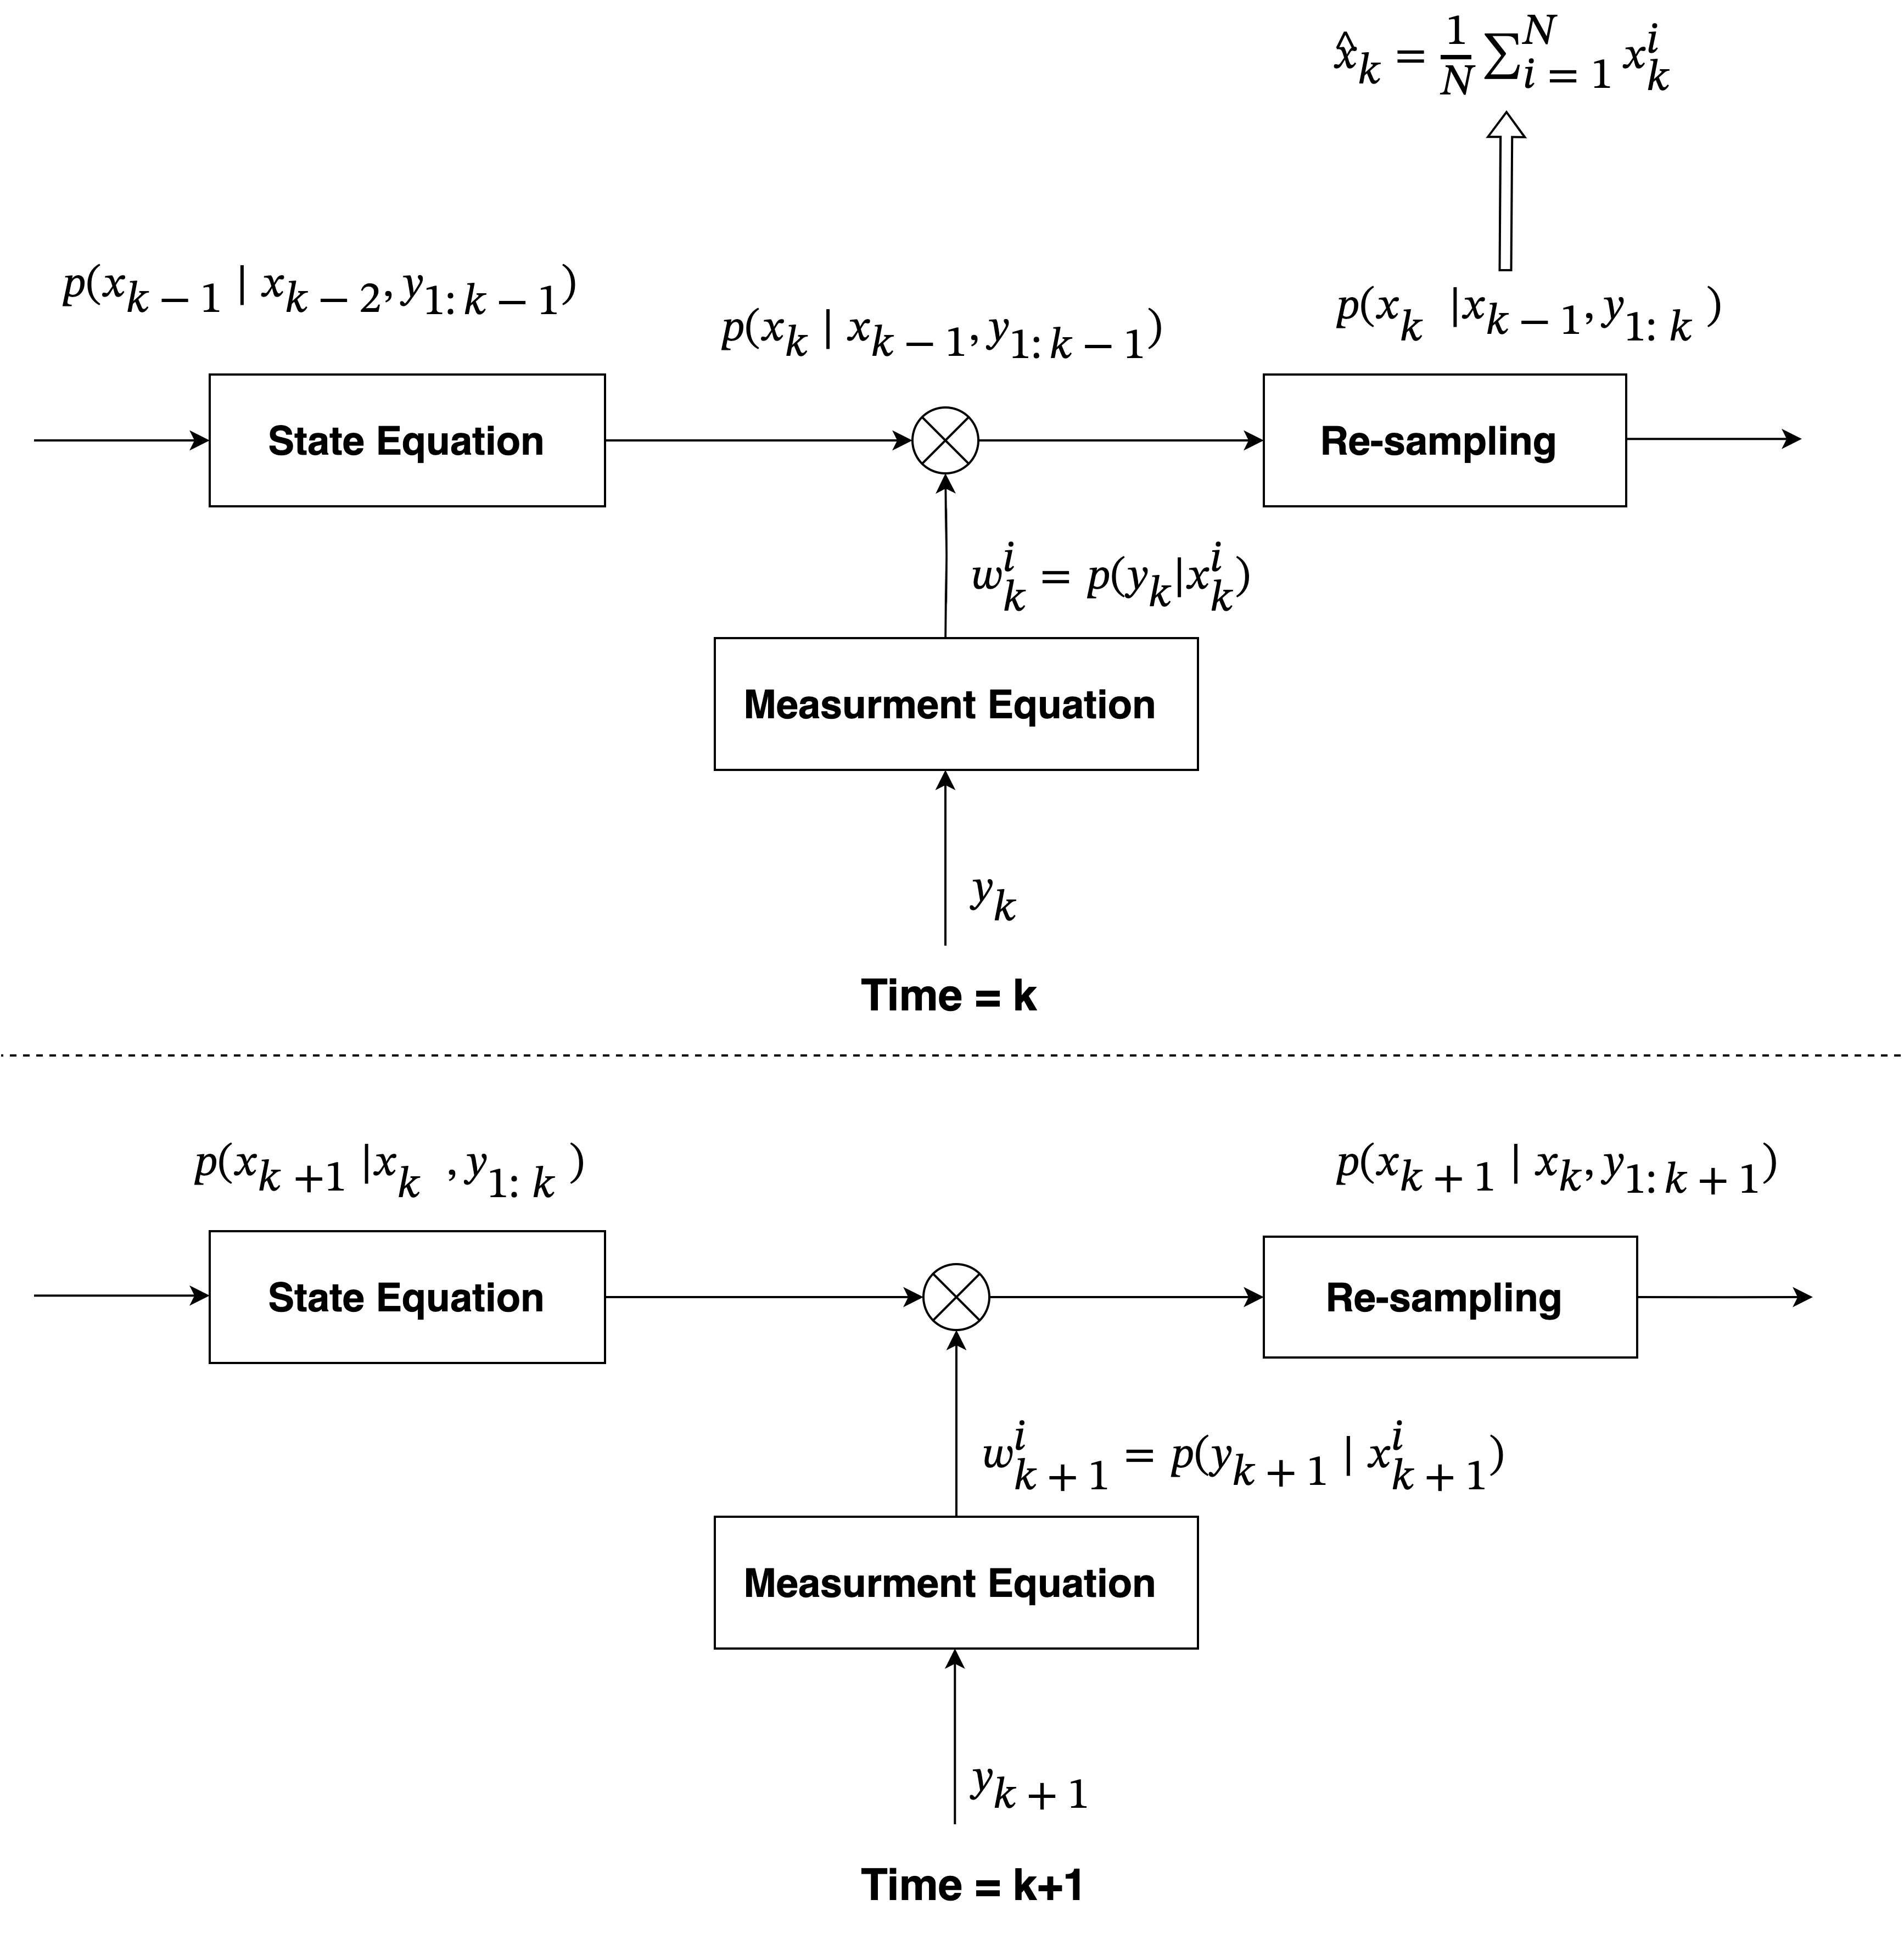
\includegraphics[width=0.75\linewidth]{Figure/SIR1.PNG}
	\caption{Implementation steps of the SIR algorithm.}
        \label{SIR}
\end{figure}

The likelihood calculation for the weights using the measurements is shown in Figure \ref{SIR}. Furthermore, the mean estimate \(\hat{x}_k\) is calculated using the average value. By using  Equation (\ref{352}) to check the number of effective particles, a decision to resample or not can be made at each update, thereby reducing computational load when resampling is unnecessary. In the resampling stage, the less effective particles are replaced by particles with higher weights, ensuring that there is a significant number of particles that accurately represent the state. The algorithm for the \ac{SIR} \ac{PF} is illustrated in Algorithm\ref{alg:particle_filter}.\footnote{The Matlab code for the algorithm's implementation can be found in the code repository from Appendix \ref{appendix:repo}.}


\begin{algorithm}[H]
\caption{Particle Filter Algorithm}
\label{alg:particle_filter}
\begin{algorithmic}[1]
    \vspace{2em}
    \State \textbf{Initialize:}  $\hat{x}_0$,  $\mathbf{Q}$, $\mathbf{R}$, $N$,
    \vspace{0.3em}
    \State $\mathbf{x}_i \sim \mathcal{N}(\hat{x}_0, \mathbf{Q})$, $i \gets 1, \ldots, N$
    \vspace{0.3em}
    \State $w_i \gets \frac{1}{N}$, $i \gets 1, \ldots, N$
    \vspace{1em}
    
    \State \textbf{Prediction:}
    \vspace{1em}
    \For{$i \gets 1$ to $N$}
        \State $\mathbf{x}_i \gets \mathbf{F}(\mathbf{x}_i) + \text{noise}$
        \vspace{0.3em}
        \State $\text{noise} \sim \mathcal{N}(0, \mathbf{Q})$
        \vspace{1em}
    \EndFor
    \vspace{1em}
    
    \State \textbf{Update:}
    \vspace{1em}
    \If{$z_k$ available}
        \vspace{0.5em}
        \For{$i \gets 1$ to $N$}
            \vspace{0.5em}
            \State $p(z_k \mid \mathbf{x}_i) \gets \frac{1}{\sqrt{2 \pi \sigma_{meas}^2}} \exp\left(-\frac{(z_k - h(\mathbf{x}_i))^2}{2 \sigma_{meas}^2}\right)$
            \vspace{0.3em}
            \State $w_i \gets w_i \cdot p(z_k \mid \mathbf{x}_i)$
            \vspace{0.3em}
        \EndFor
        \vspace{0.5em}
        \State $w_i \gets \frac{w_i}{\sum_{j=1}^N w_j}$ for all $i \gets 1, \ldots, N$
    \EndIf
    \vspace{1em}
    
    \State \textbf{Systematic Resampling:}
    \vspace{1em}
    \State $N_{\text{eff}} \gets \frac{1}{\sum_{i=1}^N w_i^2}$
    \vspace{0.5em}
    \If{$N_{\text{eff}} < \frac{N}{2}$}
        \vspace{0.5em}
        \State $\text{cumulative\_weights} \gets \text{cumsum}(w_i)$
        \vspace{0.3em}
        \State $\text{thresholds} \gets \text{linspace}(0, 1 - 1/N, N) + \text{rand}(1, N)/N$
        \vspace{0.3em}
        \For{$i \gets 1$ to $N$}
            \vspace{0.3em}
            \State Find index $j$ such that $\text{thresholds}[i] \le \text{cumulative\_weights}[j]$
            \vspace{0.3em}
            \State $indexes[i] \gets j$
        \EndFor
        \vspace{0.5em}
        \State $\mathbf{x}_i \gets \mathbf{x}_{indexes[i]}$
        \State $w_i \gets \frac{1}{N}$
    \EndIf
    \vspace{1em}
    
    \State \textbf{Estimation:}
    \vspace{1em}
    \For{$i \gets 1$ to $N$}
        \vspace{0.5em}
        \State $\hat{x}_k \gets \hat{x}_k + w_i \mathbf{x}_i$
        \vspace{0.5em}
    \EndFor
    \vspace{1em}
\end{algorithmic}
\end{algorithm}

\section{Adaptive Filtering Theory}
Accurate state estimation is crucial for the performance of tracking filters. The covariance matrices of measurement noise $\mathbf{R}$ and process noise $\mathbf{Q}$ play a significant role in the effectiveness of these filters. To maintain optimal filter performance, these matrices may need to be adjusted dynamically based on the specific use case. Most tracking filters generally perform well when the target behaves according to the assumed process model. However, they can struggle when there are deviations from this model or unexpected events not accounted for by the model. For example, if a filter is designed to track a target moving at a constant velocity with occasional speed changes, it will typically perform well. But if the target suddenly manoeuvres or changes speed in a manner not predicted by the model, the filter's performance may degrade.

Also the presence of outliers in the observations that significantly deviate from the expected distribution can adversely affect filter accuracy. Filters like the Kalman Filter and the \ac{UKF}, which rely on Gaussian assumptions, are particularly sensitive to such deviations. If an observation falls within the tracking gate but deviates significantly from the expected distribution, it can lead to poor estimations. In the context of tracking commercial aircraft, where sudden maneuvers are not anticipated and robust estimations are crucial, it is essential for the filter to handle deviations and outliers effectively. Adjusting the covariance matrices dynamically can help maintain the robustness and accuracy of the filter under varying conditions.
\newline
\newline
According to Mehra \cite{Mehra1972}, approaches to adaptive filtering can be categorized into four types: Bayesian, maximum likelihood (ML), correlation, and covariance matching. In the approach to tracking commercial aircraft for this project, the focus will be on utilizing covariance matching methods for adaptive filtering.

\subsection{Covariance Scaling Theory}
The covariance scaling method focuses on scaling the matrix of the innovation or residual based on their theoretical values. Similarly to the approach introduced in \cite{Akhlaghi2018}, the method for tuning the covariance matrices is discussed. The innovation value and the residual value equations are shown in (\ref{dk}) and (\ref{ek}) respectively which are used for adjusting the covariance matrices.
\begin{equation}
    d_k = \left[ z_k - h_k(\hat{X^-_k})\right]
    \label{dk}
\end{equation}
\begin{equation}
    \varepsilon_k = \left[ z_k - h_k(\hat{X^+_k})\right]
    \label{ek}
\end{equation}
Where \(z_k\) is the measurement and the \(\hat{X}^-_k\) is the predicted state and  \(\hat{X}^+_k\) is the estimated state at time \(k\).Using these values, the measurement covariance matrix \(\mathbf{R}\) and process noise covariance matrix \(\mathbf{Q}\) can be scaled accordingly.

\subsubsection{Adaptive Estimation of \( R \)}

The innovation covariance matrix of the tracking filter at time \( k \) is defined as:

\begin{equation}
    S_k = H_k P^-_k H^T_k + R_k
\end{equation}

where \( H_k \) is the measurement mapping matrix and \( P^-_k \) is the predicted error covariance matrix at time \( k \). The measurement covariance matrix \( R_k \) can be rewritten as:

\begin{equation}
    R_k = S_k - H_k P_k H^T_k
\end{equation}

Theoretically, \( R_k \) should be a positive definite matrix to ensure that the measurement covariance matrix represents a valid probability distribution with non-negative variances. Using the approach from \cite{wang1999stochastic}, \( R_k \) can be estimated by:

\begin{equation}
    \bar{S_k} = \mathbb{E}\left[ \varepsilon_k \varepsilon_k^T \right] 
    \label{357}
\end{equation}

\begin{equation}
    R_k = \mathbb{E}\left[ \varepsilon_k \varepsilon_k^T \right] + H_k P^-_k H_k^T 
    \label{358}
\end{equation}

To implement what is shown in Equation (\ref{358}), the expectation operation of \(\varepsilon_k \varepsilon_k^T\) is approximated by averaging \(\varepsilon_k \varepsilon_k^T\) over time. A moving window with previous residuals is used, or a forgetting factor, similar to the one introduced in \cite{Akhlaghi2018}, can be applied where \(0 \le \alpha \le 1\). A larger value of \(\alpha\) can be used to adaptively estimate \(R_k\) to incur fewer fluctuations and longer time delays when dealing with abrupt changes. The following equation applies:

\begin{equation}
    R_k = \alpha R_{k-1} + (1-\alpha)(\varepsilon_k \varepsilon_k^T + H_k P^-_k H_k^T)
    \label{time_delays}
\end{equation}

At every update, instead of using the normal measurement covariance matrix, the one derived in Equation (\ref{time_delays}) is used for adaptive estimation. Alternatively, the process noise covariance matrix \(Q\) can be adapted when dealing with abrupt changes or outliers in the observations.

\subsubsection{Adaptive Estimation of \( Q \)}

To scale the process noise covariance \( Q \), an approach similar to that proposed in \cite{Ding2007} can be used. For an optimal filter, the predicted innovation covariance matrix should match the one computed from the innovation sequence, as demonstrated in Equation (\ref{357}). Directly resolving \( P^-_k \) from equation(\ref{358}) is not straightforward. Therefore, a simpler method based on the scaling factor introduced in \cite{Ding2007} is used.

The scaling factor \( \alpha \) is defined as:

\begin{equation}
    \alpha = \frac{\text{trace}\{H_k \tilde{P}^-_k H_k^T\}}{\text{trace}\{H_k \hat{P}^-_k H_k^T\}} = \frac{\text{trace}\{\varepsilon_k \varepsilon_k^T - R_k\}}{\text{trace}\{H_k \hat{P}^-_k H_k^T\}}
\end{equation}

Here, \( \alpha \) adjusts the process noise covariance \( Q \) by comparing the traces of the predicted and actual innovation covariance matrices. To derive \( \alpha \), substitute the expression for \( \hat{P}^-_k \):

\begin{equation}
    \hat{P}^-_k = \Phi_{k-1} \hat{P}_{k-1} \Phi_{k-1}^T + Q_{k-1}
\end{equation}

Substituting this into the scaling factor equation gives:

\begin{equation}
    \alpha = \frac{\text{trace}\left\{H_k \left(\Phi_{k-1} \hat{P}_{k-1} \Phi_{k-1}^T + \tilde{Q}_{k-1}\right) H_k^T\right\}}{\text{trace}\left\{H_k \left(\Phi_{k-1} \hat{P}_{k-1} \Phi_{k-1}^T + Q_{k-1}\right) H_k^T\right\}}
\end{equation}

The adaptation rule for \( Q \) is then defined as:

\begin{equation}
    \hat{Q}_k = Q_{k-1} \sqrt{\alpha}
\end{equation}

here the square root in the adaptation rule introduces a smoothing effect, helping to stabilize the adjustment of \( Q \).


\section{Log-Likelihood Statistical Benchmark}

The likelihood function, in probabilistic terms, expresses how probable the observed data is given a set of model parameters. For a given observation \( z_k \) and state prediction \( Hx_k \), the likelihood \( L \) represents the probability of observing \( z_k \), assuming the predicted state \( Hx_k \) and the associated uncertainties in the system. Mathematically, this can be expressed as:

\begin{equation}
    L(z_k | Hx_k) = p(z_k | Hx_k, P, R)
\end{equation}

where \( P \) is the state covariance matrix and \( R \) is the measurement noise covariance matrix. 

The log-likelihood, which is the natural logarithm of the likelihood function as discussed in the literature review, simplifies this expression and is widely used due to its mathematical convenience in optimization and statistical inference \cite{Grewal2006}. For instance, the likelihood for the Kalman Filter residual \( e_k = z_k - Hx_k \), given the system uncertainty \( S = HPH^\top + R \), is expressed as:

\begin{equation}
    L = \frac{1}{\sqrt{2\pi S}} \exp\left( -\frac{1}{2} e_k^\top S^{-1} e_k \right)
    \label{eqLikelihood}
\end{equation}

Taking the natural logarithm of the likelihood, Equation (\ref{eqLogLikelihood}) can be obtained.

\begin{equation}
    \log(L) = -\frac{1}{2} \left( \log(2\pi S) + e_k^\top S^{-1} e_k \right)
    \label{eqLogLikelihood}
\end{equation}

This function evaluates how well the predicted observations align with the actual observations while accounting for uncertainties in both the system and measurements. The log-likelihood offers several advantages, with the main advantage being that the logarithm is a strictly increasing function, meaning it reaches its maximum at the same point as the original likelihood function \cite{labbe2014kalman}.
\newline
\newline
The log-likelihood is related to performance measures such as the \ac{NIS} and the \ac{NEES}, which are widely used to evaluate the accuracy and consistency of tracking filters, as noted in the literature review section.
\newline
The \textit{NEES} is given by:
\begin{equation}
    \epsilon_{x,k} = e_{x,k}^\top P^{-1}_{k|k} e_{x,k}
\end{equation}

where \( e_{x,k} \) is the estimation error between the true state and the predicted state, and \( P_{k|k} \) is the covariance matrix of the estimated state. The \ac{NEES} metric evaluates the accuracy of state estimates by comparing them to the true state of the system. Since calculating \ac{NEES} depends on knowing the true state \( x_k \), it is generally applied in simulation environments or in cases where an external validation system is available \cite{chen2024kalman}.
\newline
The \textit{NIS}, on the other hand, is computed as:
\begin{equation}
    \epsilon_{z,k} = e_k^\top S^{-1}_{k|k-1} e_k
\end{equation}
where \( e_k = z_k - Hx_k \) is the innovation vector, and \( S_{k|k-1} \) is the innovation covariance matrix. Unlike \ac{NEES}, \ac{NIS} does not require ground truth information; it only depends on the observation sequence, making it more suitable for real-world data without access to the true state \cite{chen2018weak}. The performance evaluation performed on the tracking filters in the next chapters focuses on the Log-likelihood function to evaluate the tracking filters due to its ability to provide a direct measure of model fit based on probability theory




\section{Conclusions}
In this chapter, a theoretical study of various tracking filters, adaptive filtering methods, and tracking filter performance was presented, with a focus on their mathematical foundations. The discussion began with an introduction to state-estimation theory, followed by the theory of the tracking filters, including the Kalman Filter, the \ac{UKF}, the \ac{SIR} Particle Filter, and the \ac{RGNF}. This section elucidated their underlying principles, mathematical formulations, and algorithms for use in state estimation of dynamic systems. Additionally, an overview of adaptive filtering methods, particularly those involving covariance scaling were presented. Lastly, the log-likelihood was introduced as a statistical benchmark for performance evaluation.

The next chapter will focus on simulations, implementing the discussed tracking filters, and validating them through simulated aircraft trajectories in the bistatic range and Doppler domains. The performance of the tracking filters will be evaluated using various metrics, including the log-likelihood, to compare their effectiveness in various scenarios.
